\documentclass[leqno,11pt]{book}
\usepackage{amsfonts,amssymb,amsmath,longtable,array,bbm,url}
\usepackage[utf8]{inputenc}
\usepackage[T2A]{fontenc}
\usepackage[english]{babel}
\usepackage{amssymb}
\usepackage{graphicx}
\usepackage{epstopdf}
\usepackage{float}
\usepackage{wrapfig}

\newenvironment{proof}{{P\,r\,o\,o\,f. }}{~~~{$\Box$}}
%\usepackage{serd_inf}
%\usepackage{fancyhea}
\usepackage{enumerate}
\usepackage[dvips]{epsfig}

\newcommand{\rf}[1]{(\ref{#1})}
\newcommand{\RR}{\mathbb{R}}

\renewcommand{\thesubsection}{}
\makeatletter
\def\@seccntformat#1{\@ifundefined{#1@cntformat}%
   {\csname the#1\endcsname\quad}%    default
   {\csname #1@cntformat\endcsname}}% enable individual control
\newcommand\section@cntformat{}     % section level 
\makeatother

\newtheorem{definition}{Definition}
\newtheorem{construction}{Construction}
\newtheorem{example}{Example}
\newtheorem{proposition}{Proposition}
\newtheorem{lemma}{Lemma}
\newtheorem{theorem}{Theorem}

\def\p{\phantom{0}}
\everymath{\displaystyle}
\allowdisplaybreaks

\def\theequation{\arabic{equation}}

\def\hlst{\setlength{\topsep}{4pt}\setlength{\partopsep}{4pt}%
\setlength{\parsep}{4pt}\setlength{\itemsep}{\parskip}}
%\begin{list}{{$\bullet$}}{\hlst}

%\setlength{\textfloatsep}{3pt}
%\setlength{\floatsep}{3pt}
%\setlength{\intextsep}{3pt}
\newcommand{\eeth}{\rm}
\newcommand{\dO}{\partial\Omega_{h}}
%%%%%
\textwidth 13.5cm
\textheight 18.5cm
\topmargin 0in
\parindent 0.5in
%\headsep 0in
\oddsidemargin 0.5in
\evensidemargin 0.5in

\makeatletter
\def\ps@serdica{%
    \let\@oddfoot\@empty\let\@evenfoot\@empty
    \def\@evenhead{\thepage\hfil{\sl \leftmark} \hfil}%
    \def\@oddhead{\hfil{\sl \rightmark}\hfil\thepage}%

    }
\makeatother

\pagestyle{serdica}

\newcommand\kwams[2]
{
\def\thefootnote{}
\footnote{{\it$\rm{}$}
#1

{}~~{\it Key words:} #2
}
}

\def\abstractname{} %{\sc Abstract.}} % <---------
\def\abstract{\if@twocolumn
\section*{\abstractname}
\else \small
%\begin{center}
%{\abstractname} %\vspace{-.5em}\vspace{0pt}}
%\end{center}
%\noindent
\quotation  \noindent
\fi}
\def\endabstract{\if@twocolumn\else\endquotation\fi}

\def\bibname{\rm R\,E\,F\,E\,R\,E\,N\,C\,E\,S} % <----------
\def\thebibliography#1{\addvspace{3em}\noindent
\hfil \bibname \hfill \list
 {[\arabic{enumi}]}{\settowidth\labelwidth{[#1]}\leftmargin\labelwidth
 \advance\leftmargin\labelsep
 \usecounter{enumi}}
 \def\newblock{\hskip .11em plus .33em minus .07em}
 \sloppy\clubpenalty4000\widowpenalty4000
 \sfcode`\.=1000\relax}
\let\endthebibliography=\endlist

\newcommand{\head}[8]
{ % 1-page, 2-title, 3-author, 4-short title,
  % 5-author, 6-vol, 7-year, 8-number
\thispagestyle{empty}

\noindent {\footnotesize{\rm Serdica} J. Computing {\bf #6} (#7),
No #8, #1} \hfill
%\begin{minipage}{42mm}
\setlength{\unitlength}{1mm}
\begin{picture}(46,14.13)
%%%\put(0,2.5){\special{em:graph serd-inf.bmp}} %3
%\put(54.6,1.9){\special{em:graph serd1o.pcx}}
\end{picture}
%\end{minipage}

\vspace*{2cm}

\markboth{#5}{#4} \vspace*{2cm}
\begin{center}
{\large\bf #2}  %%%\uppercase{#2}}

\bigskip

{\large #3}

\end{center}

\bigskip

\bigskip
}

\newcommand{\sect}[1]{\bigskip \par {\large\bf #1}}

%%%%%


\begin{document}
\setcounter{page}{3}

\def\thefootnote{}
\footnote{{\it ACM Computing Classification System $\rm(1998){ G.1.8, G.1.10}$}
%#1

{}~~{\it Key words:} two dimensional Boussinesq equation, traveling wave solutions (TWS), high order finite difference schemes, asymptotic boundary conditions
}

\head{3--4} {
Numerical Study of Soliton Solutions to the Two Dimensional Boussinesq  Equation
}
{K. Angelow, N. Kolkovska}
{
}
{K. Angelow, N. Kolkovska} {8}{2018}{2}

{\centering
\small \sl

}

\bigskip

\begin{abstract}\noindent{\sc Abstract.}
The aim of this paper is to evaluate propagating  wave solutions to the two dimensional Boussinesq Equation (BE). To solve this nonlinear fourth order hyperbolic  problem we use high order finite difference schemes for the spatial derivatives. Taylor Series (TS) expansion is used to describe the time derivatives. A Boundary Condition (BC) is applied on the computational boundary. Results from the TS approach are compared with results from another known method in the literature. The performed numerical tests exhibit good convergence and confirm the validity of the TS method.

\footnotetext{*This work is supported by the Institute of Mathematics and Informatics, Bulgarian
Academy of Sciences. The second author is partially supported by the Bulgarian Science Fund under  Grant~H~22/2 from 2018.}
\end{abstract}
\bigskip
\setcounter{footnote}{0}
\def\thefootnote{\arabic{footnote}}

\sect{1.~Introduction.}\label{introduction}

In this paper we  consider the two dimensional Boussinesq  Equation (BE)
\begin{align} \label{eq1}
&u_{tt} - \Delta u -\beta_1  \Delta u_{tt} +\beta_2 \Delta ^2 u + \Delta f(u)=0   \quad \text{for}  (x,y) \in \RR^2, \, t\in\RR^+, 
\\ \nonumber &u(x,y,0)=u_0(x,y), \, u_t(x,y,0)=u_1(x,y)   \quad\text{for} \, (x,y) \in \RR^2,
\\  &u(x,y) \rightarrow 0,  \Delta u(x,y) \rightarrow 0 ,  \quad \text{for}  \sqrt{x^2 + y^2} \rightarrow \infty, \label{eq11}
\end{align}
where   $f(u)=\alpha u^2$,  $\alpha>0$, $\beta_1>0$, $\beta_2>0$  are dispersion parameters, and $\Delta$ is the Laplace operator. The BE is famous with the approximation of shallow water waves or also weakly non--linear long waves. It is often used for simulation of various physical processes e.g. turbulence in fluid mechanics, vibrations in acoustics etc. A derivation of the BE from the original Boussinesq system can be found in \cite{ChChr}.

The goal of the article is to seek for soliton solutions to \rf{eq1}, which 
are traveling  in $y$ direction with velocity $c$. The most suitable Initial Condition (IC) for the numerical solver of the hyperbolic BE \rf{eq1} -- \rf{eq11} that was developed here, is found in \cite{EllipticProblem}. TS expansion is used to calculate the next time layer with respect to the time step $\tau$. The time derivatives
are obtained from the main equation by an iterative procedure. This is possible because the equation allows to isolate the highest time derivative on one side of the equation. By differentiating with respect to time variable one could obtain higher time derivative terms in the TS expansion. Thus the solver could be adjusted to use second, fourth or sixth approximation order, i.e. $O(\tau^2)$, $O(\tau^4)$, $O(\tau^6)$. To increase the precision of the numerical method, finite difference schemes (FDS) with local approximation of forth $O(h^4)$ and sixth $O(h^6)$ order are applied to the spatial derivatives i.e. the second derivative along space are approximated with high order finite differences. Thus the numerical solution is computed on relatively coarse grid with high accuracy. In order to compare the results from TS method, a conservative finite difference scheme with weights is used, which applies second order of approximation along time and space.
Both methods are tested with zero boundary and also with BC found and developed in \cite{BoundaryProblem}.

\sect{2.~Taylor Series Approach for the BE in Two Dimensions}\label{TaylorA}

The following variable change
\begin{equation}\label{vc}
x = \sqrt{\beta_1} \tilde x, \quad y = \sqrt{\beta_1} \tilde y, \quad t = \sqrt{\beta_1} \tilde t, \quad \tilde \Delta = \tilde u_{\tilde x \tilde x} + \tilde u_{\tilde y \tilde y}
\end{equation}
transforms the main equation \rf{eq1}  into 


\begin{equation}\label{eqVC}
(E-\tilde \Delta)  \tilde u_{\tilde t \tilde t} = \frac{(E-\tilde\Delta)\tilde\Delta \tilde u + \alpha \beta \tilde\Delta(\tilde u^2) + (\beta -1)\tilde\Delta \tilde u}{\beta},
\end{equation}
where $\beta = \beta_1 / \beta_2$.
Revert to old abbreviations $x$, $y$, $t$ and $u$ and define $L$ to be an operator of the form
\begin{equation}\label{operator}
Lu = \frac{\Delta u + (E-\Delta)^{-1} ( \alpha \beta \Delta( u^2) + (\beta -1)\Delta u)}{\beta},
\end{equation}
where the negative power denotes the inverse operator of $(E-\Delta)$. The finite differences along time and space require TS expansions of $u(x,y,t)$. Therefore it is assumed that the solution is $s$ times infinitely differentiable with respect to $t$ and $p$ times infinitely differentiable with respect to $x$ and $y$, i.e. $u \in C^s(I, R)$ and $u \in C^p(\Omega, R)$. For simplicity $s$ also stands for the order of the TS expansion and $p$ stands for the order of the FDS approximations along the computational box $\Omega_h$. It is shown that the error of the method is $O(h^p + \tau^s)$ if a suitable boundary condition is applied on $\partial \Omega_h$.

If the two dimensional differential operator $(E-\Delta)$ is discretized numerically by finite differences then it can be inverted using Fast Poisson Solvers \cite{FPS}. The last algorithm produces band matrices which need to be inverted. Thomas algorithm is used for three diagonal matrices and $O(h^2)$ approximation order.  Five and seven diagonal matrices (with $O(h^4)$ and $O(h^6)$ approximation order, respectively) use similar to Thomas technique which is again a simplified form of Gauss elimination.

A function $u$ is defined by $u : \bar \Omega \times T \rightarrow  R^2$. If $\Omega_h$ is the corresponding grid to $\Omega$ then $u_h$ is defined as the restriction of $u$ over $\Omega_h$
$$u_h : \bar \Omega_h \times T \rightarrow  R$$
$$ (x,y) \in \bar \Omega_h \rightarrow u_h(x,y, t_k)$$
for arbitrary $t_k \in T$.

Thus an explicit formula for the highest derivative of $u$ in PDE \rf{eqVC} 

\begin{equation}\label{Leq}
\frac{ \partial^2 u_h }{ \partial t^2 } = L_h u_h = \frac{ \Delta_h u_h + (E - \Delta_h)^{-1} ( \alpha \beta \Delta_h( u_h^2) + (\beta -1)\Delta_h u_h) }{\beta}
\end{equation}
is obtained. It is supposed that the solution is $s$ times differentiable on $T$ thus the last transforms into

\begin{equation}\label{DLeq}
D^{\tilde s} (u_h) =\frac{ \Delta_h D^{\tilde s - 2}(u_h) + (E - \Delta_h)^{-1}( \Delta_h D^{\tilde s - 2} ( \alpha \beta u_h^2  + (\beta -1)u_h) )  }{\beta} 
\end{equation}

with $D^{(\tilde s)} := \partial^{\tilde s} / \partial t^{\tilde s}$ and $\tilde s = 2,...,s$. The $\tilde s^{th}$ time derivative requires $(\tilde s-2)^{th}$, $(\tilde s-3)^{th}$, ..., $2^{nd}$ and $1^{st}$ derivatives and the function $u_h$ itself. E.g. if one would like to calculate the $7^{th}$ derivative $\partial^7 u / \partial t^7$, then $5^{th}$, $4^{th}$, $3^{rd}$, $2^{nd}$, $1^{st}$ and $0^{th}$ derivatives are used and the $5^{th}$ requires  $3^{rd}$, $2^{nd}$, $1^{st}$ and $0^{th}$ and so on.  Thus if $\psi$ and $\bar \psi$ are two known functions with $\psi(x,y) = u(x,y, t_k)$ and $\bar \psi(x,y) = u_t(x,y, t_k)$ then the derivative $\partial^{\tilde s} u / \partial t^{\tilde s}$ could be expressed solely by $\psi$ and $\bar \psi$ at $t = t_k$. Let's define the following function set

\begin{equation}
Q_{\tilde s}(u_h) := \{ D^{q}(u_h), q = 0, ... , \tilde s - 2 \}.
\end{equation}
In order to describe the iterative process in short notations the following vector valued functions are defined
\begin{align*} 
P_{\tilde s} : \Omega_h^{(\tilde s - 1)} \rightarrow \Omega_h
\\ Q_{\tilde s}(u_h(t_k)) \rightarrow P_{\tilde s} (Q_{\tilde s}(u_h) ) = L_h( D^{(\tilde s - 2)} (u_h(t_k)) ).
\end{align*}

Example 1. The PDE \rf{eqVC} can be expressed through 
\begin{equation}\label{example}
D^{2}(u_h) = P_0(Q_0(u)) + O(h^p) = P_0(u_h) + O(h^p),
\end{equation}
which is equation \rf{Leq} written in short form. When the operator $D^{(\tilde s -2)}$ is applied on both sides of equation \rf{example}, it follows that
\begin{equation}\label{DPeq}
D^{\tilde s}(u_h) = P_{\tilde s}(Q_{\tilde s}(u)) + O(h^p))
\end{equation}
which is the short form of \rf{DLeq}. Now let $\tilde s = 6$, then \rf{DPeq} reads as

\begin{align*} 
D^6 u_h - O(h^p) = P_4(Q_4(u_h)) =
\\
= P_4(\{u_{ h}, u_{ h_{t} }, u_{ h_{tt} }, u_{ h_{ttt} }, u_{ h_{tttt} } \}) = 
\\
= P_4(\{u_{ h}, u_{ h_{t} }, P_0(\{u_h\}),  P_1( \{ u_h, u_{ h_{t} } \} ), P_2( \{ u_h, u_{ h_{t} }, u_{ h_{tt} } \} )  \}) = 
\\ 
= P_4(\{u_{ h}, u_{ h_{t} }, P_0(\{u_h\}),  P_1( \{ u_h, u_{ h_{t} } \} ), P_2( \{ u_h, u_{ h_{t} },  P_0( \{ u_h \} ) \} )  \}).
\end{align*}

Example 2. Let's look at PDE \rf{eqVC}. For $\tilde s = 2$:
$$
u_{tt} = Lu.
$$
For $\tilde s = 3$:
$$
u_{ttt} = L(D(u)) = \frac{ \Delta u_t + (E - \Delta)^{-1}           ( \Delta (2 \alpha \beta u u_t  +                          (\beta -1)u_t) )  }{\beta}.
$$
For $\tilde s = 4$:
$$
u_{tttt} = L(D^2(u)) = \frac{ \Delta u_{tt} + (E - \Delta)^{-1}( \Delta (2 \alpha \beta ( u Lu +  u_t^2 )   + (\beta -1) u_{tt} ) )  }{\beta}.
$$

A more general formula, which is relevant only to the complexity of the algorithm, i.e. to estimate the number of operations for its calculation, is

\begin{align*}
\beta LD^{(\tilde s)} u =   \Delta D^{ (\tilde s - 2) }(u)  +
\\
 (E - \Delta)^{-1}( \Delta ( \alpha \beta \sum_{j=0}^{ \tilde s - 2}  { \tilde s - 2\choose j} D^j(u) D^{ (\tilde s - 2 - j) }(u)+ (\beta -1) D^{ (\tilde s - 2) }(u) ) ).
\end{align*}
Nevertheless the formula itself is not our goal, just use the computer to derive it and evaluate it for a given function set $Q_{\tilde s}$.

The spatial  derivatives discretization in \rf{DLeq} is made by using centered finite differences and extending the stencil:
\begin{equation}\label{fd}
v_{\widehat{xx},p}(x) :=  \frac{1}{h^2} \sum\limits_{i=-p/2}^{p/2} d_i u(x+ih),
\end{equation}
 Here $p$ is equal to $2$, $4$ or $6$.  The weights $d_i$ taken from  \cite{forn} are  
 $ 1,-2,1$ for $p=2$, $-\frac{1}{12}, \frac{4}{3}, -\frac{5}{2}, \frac{4}{3}, -\frac{1}{12}$ - for $p=4$ and  $\frac{1}{90}, -\frac{3}{20}, \frac{3}{2}, -\frac{49}{18}, \frac{3}{2}, -\frac{3}{20}, \frac{1}{90}$ - for $p=6$. The approximation error of  formulae \rf{fd} is $O(h^p)$. Replacing the Laplace operator in \rf{DLeq} by the discrete Laplacian $$ \Delta_{h,p} v_{i,j} := (v_{i,j})_{\widehat{xx},p} + (v_{i,j})_{\widehat{yy},p}$$ we obtain finite difference schemes with high order of approximation $O(h^4)$ for $p=4$ and  $O(h^6)$ for $p=6 $.  The application of FDS with high order of approximation leads to a high rate of convergence of the method for sufficiently smooth solutions. In this way more accurate solutions can be produced on a coarse grid.
Till now only space discretization, with step $h$, is applied on \rf{DLeq}. Let's discretize along time domain $T$. The IC $u_0(x,y) = u(x,y,0)$ and $u_1(x,y) = u_t(x,y,0)$ are taken from \cite{EllipticProblem}. Then
$$
u_{i,j}^0 = u_{0_h}, \partial / \partial t (u_{i,j}^0) = u_{1_h}
$$
and $D^{\tilde s}(u^0)$ could be found iteratively for each $2 \leq \tilde s \leq s$ through \rf{DLeq}. If the finite difference discretizations applied along space $(E - \Delta_h)^{-1}$ and $\Delta_h )$ have order of approximation $O(h^p)$ then Taylor formula gives the following

\begin{align*}
u(x,y,\tau) = u_h^{(0)} + \tau \frac{\partial}{\partial t}(u_h^{(0)}) + ... +
\\ + \frac{\tau^s}{ s! } P_s( Q_s(u_h^{(0)}) ) + O(h^p + \tau^s) = u_h^{(1)} + O(h^p + \tau^s),
\\  \frac{\partial}{\partial t}u(x,y,\tau) = \frac{\partial}{\partial t}( u_h^{(0)}) + \tau P_2( Q_2( (\frac{\partial}{\partial t} u_h^{(0)}) ) + ... +
\\ + \frac{\tau^s}{ s! } P_{s+1}( Q_{s+1}(\frac{\partial}{\partial t}u_h^{(0)}) ) + O(h^p + \tau^s) = \frac{\partial}{\partial t}u_h^{(1)} + O(h^p + \tau^s)
\end{align*}

All derivatives on the next time layer $D^{(\tilde s) }( u_h^{(1)} )$ could be found using \rf{DLeq} because $u_h^{(1)}$ and $D^{(1) }( u_h^{(1)} )$
are already given in the last equation. Again TS could be used to find the solution at the next time layer $u_h^{(2)}$. Of course this is an iterative procedure:
\begin{align*}\label{Taylor}
u(x,y,(k+1)\tau) = u_h^{(k+1)} + O(h^p + \tau^s),
\\
u_h^{(k+1)} = u_h^{(k)} + \tau \frac{\partial}{\partial t}(u_h^{(k)}) + \sum_{ \tilde s = 2 }^{ s } \frac{ \tau^{\tilde s}}{\tilde s!} P_{\tilde s}( Q_{\tilde s}( u_h^{(k)} ) ) + O(h^p + \tau^s),
\\  
\frac{\partial}{\partial t}u(x,y,(k+1)\tau) = \frac{\partial}{\partial t}( u_h^{(k+1)}) + O(h^p + \tau^s),
\\
\frac{\partial}{\partial t}( u_h^{(k+1)}) = \frac{\partial}{\partial t}( u_h^{(k)}) + \sum_{ \tilde s = 2 }^{ s + 1 } \frac{ \tau^{\tilde s - 1}}{(\tilde s-1)!} P_{\tilde s}( Q_{\tilde s}( \frac{\partial}{\partial t} u_h^{(k)} ) )+ O(h^p + \tau^s),
\end{align*}
with approximation order $O(h^p + \tau^s)$ which is easily proved by induction. Note that the derivative set $Q_s$ at time $t_k = 0$ is calculated with approximation order $O(h^p)$ and all other sets $Q_s$ that correspond to times $t_k$, $k \in N$, are approximated with $O(h^p + \tau^s)$. At each step this numerical procedure calculates TS expansions of two numerical values: $u_h$ and its first derivative $D(u_h)$, because the PDE is of second order in time. The complexity of the algorithm depends on the order and type of the time derivatives $D^{(\tilde s)}(u_h)$ in the PDE.

The IC developed in \rf{EllipticProblem} for equation 
The following boundary function
\begin{equation}\label{eqBCV}
\widehat U_B(x , y, t) = \mu_u \frac{ (1 - \tilde c^2/\beta) x^2 - y^2}{( (1 - \tilde c^2/\beta) x^2 + y^2)^2}
\end{equation}
found in \cite{BoundaryProblem} is used to solve the stationary elliptic problem described in \cite{BoundaryProblem}.
Near  the computational boundaries $(x,y):x=L_x$ and $(x,y):y=L_y$ we do not change the stencil as described in \rf{fd}. The discrete Laplacian
is defined there by using the values of the discrete solution
\begin{equation}\label{eqBCV}
\widehat U_B(x , y, t) = \mu_u \frac{ (1 - c^2) x^2 - (y-ct)^2}{( (1 - c^2) x^2 + (y-ct)^2)^2}
\end{equation}
found in \cite{BoundaryProblem} at points outside the computational domain. The value of $\mu_u$ is obtained again from the method developed in \cite{BoundaryProblem}. For $p=2$ the second derivative $\partial^2 / \partial x^2$ is approximated with three points (green color) and uses one point outside the computational domain $\Omega_h$. For $p=4$, the derivative $\partial^2 / \partial x^2$ implies five point stencil (blue color) with maximum
\begin{wrapfigure}{r}{0.5\textwidth}
     \begin{center}
     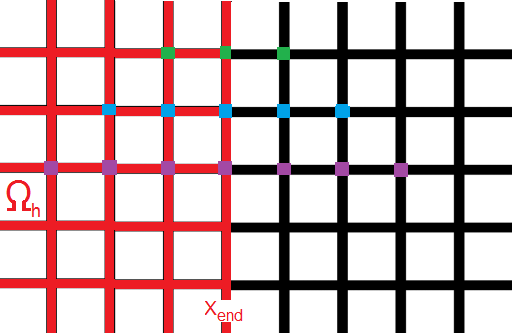
\includegraphics[scale=0.5]{Pictures/BoundaryPicture.png}
     \end{center}
	\caption{Finite Differences near the computational boundary.}
	\label{fig:BoundaryFD}
\end{wrapfigure}
two extra points and for $p=6$ it implies seven point stencil (purple color) with maximum three extra points outside the computational domain $\Omega_h$ (see Figure \ref{fig:BoundaryFD}). Same reasoning is implied for the $\partial^2 / \partial y^2$ derivative. The affected terms in equation \rf{Leq} which make use of the boundary function \rf{eqBCV} are the following:
\begin{equation*}
\frac{ \Delta_h u_h}{\beta}, \frac{ (E - \Delta_h)^{-1} ( (\beta -1)\Delta_h u_h) }{\beta}
\end{equation*}
The TS approach also requires time derivatives of both terms defined above
\begin{equation*}
\frac{ \Delta_h D^{(\tilde s)} (u_h)}{\beta}, \frac{ (E - \Delta_h)^{-1} ( (\beta -1)\Delta_h D^{(\tilde s)}(u_h) ) }{\beta}
\end{equation*}
for $\tilde s = 0, ..., s-2$.  Thus, $D^{\tilde s}(\widehat U_B(x , y, t))$  time derivative values outside the computational boundary $\partial \Omega_h$ are also used to extend the $p+1$ point stencil where needed (see Figure  \ref{fig:BoundaryFD}).


\frenchspacing
\def\bibname{\rm R\,E\,F\,E\,R\,E\,N\,C\,E\,S}
\begin{thebibliography}{30}

%1
\bibitem{ChChr} C.I. Christov, An energy-consistent dispersive shallow-water model,  {\it Wave Motion}, \textbf{34} (2001), 161-174.

%2
\bibitem{EllipticProblem}
K. Angelow, N. Kolkovska, Numerical Study of Traveling Wave Solutions to 2D Boussinesq Equation.
Serdica J. Computing,  8, (2018) 3-4.

%3
\bibitem{BoundaryProblem}
K. Angelow, New Boundary Condition for the Two Dimensional Stationary Boussinesq Paradigm Equation.
International Journal of Applied Mathematics, (2018).

%4
\bibitem{FPS}
T. Lyche, Fast Poisson Solvers and FFT, Lecture Notes, University of Oslo, Norway

%5
\bibitem{chr-chr-07}
M.~Christou, C.~I.~Christov, Fourier–Galerkin method for 2D solitons of Boussinesq equation, 
Mathematics and Computers in Simulation, 74, (2007) 82 -- 92.
%6
\bibitem{chr-chr}
M.~Christou, C.~I.~Christov, Galerkin Spectral Method for the 2D Solitary
Waves of Boussinesq Paradigm Equation, CP 1186, (2009) 217 -- 225.
%7
\bibitem{Ch2012}
C.~I.~Christov,  Numerical implementation of the asymptotic boundary conditions
for steadily propagating 2D solitons of   Boussinesq type equation,       
Math. Computers  Simul., 82 (2012),  1079 -- 1092.
%8
\bibitem{Ch2011}
C.~I.~Christov, J. Choudhury, Perturbation solution  for the 2D Boussinesq equation,       
Mech. Res. Commun., 38 (2011),  274 -- 281.
%9
\bibitem{cher}
A.~Chertock, C.~Christov, A.~Kurganov, Central--upwind schemes for the  Boussinesq paradigm equation, Comp. Sci. High Performance Comp. IV, NNFM, 113, (2011), 267 -- 281.

\bibitem{dani}
C.~Christov, N.~Kolkovska, D.~Vasileva, On the numerical simulation of unsteady solutions for the 2D Boussinesq paradigm equation, LNCS, 6046  (2011), 386 -- 394.

\bibitem{chd-chr}
J.~Choudhury, C.~Christov, 2D  Solitary waves of  Boussinesq equation, CP75, (2005), 85 -- 90.
 
\bibitem{bnd}
K.~Angelow, New Boundary Condition for the Two Dimensional Stationary Boussinesq Paradigm Equation, 
International Journal of Applied Mathematics, Vol. 32, No 1, (2019), 141 -- 154.

\bibitem{forn}
B.~Fornberg, Generation of Finite Difference Formulas on Arbitrarily Spaced Grids, 
Math. Comput., 51(1988),  699 -- 706.

\bibitem{sam}
A.~Samarskii, The theory of difference schemes, M. Dekker,  2001.

\end{thebibliography}

\bigskip
\noindent\sl
\begin{tabular}[b]{l}
Krassimir Angelow\\
Institute of Mathematics and Informatics\\
Bulgarian Academy of Sciences, Acad.\\
G.~Bonchev Bl.8, 1113, Sofia,
Bulgaria\\
e-mail: \texttt{angelow@math.bas.bg}\\
\\
Natalia Kolkovska\\
Institute of Mathematics and Informatics\\
Bulgarian Academy of Sciences, Acad.\\
G.~Bonchev Bl.8, 1113, Sofia,
Bulgaria\\
e-mail: \texttt{n.kolkovska@gmail.com}
\end{tabular}
\hfill
\begin{tabular}[b]{l}
Received ...\\
Final Accepted ...
\end{tabular}

\end{document}
